\documentclass[11pt,a4paper]{article}

\usepackage[utf8]{inputenc}
\usepackage[T1]{fontenc}
\usepackage{lmodern}
\usepackage[english]{babel}
\usepackage[margin=2.3cm]{geometry}
\usepackage{microtype}
\usepackage{parskip}
\usepackage{enumitem}
\usepackage{hyperref}
\usepackage[table]{xcolor}
\usepackage{listings}
\usepackage{booktabs}
\usepackage{graphicx}
\usepackage{titling}
\usepackage{tikz}
\usepackage{fancyhdr}
\usetikzlibrary{arrows.meta,positioning,shapes.geometric,calc,fit,backgrounds}

\definecolor{gsuyellow}{HTML}{D4A017}
\definecolor{gsublue}{HTML}{1F4E79}
\definecolor{softgray}{HTML}{F4F4F6}
\definecolor{accentgreen}{HTML}{2E7D32}
\definecolor{accentred}{HTML}{C62828}

\hypersetup{
    colorlinks=true,
    linkcolor=gsublue,
    urlcolor=gsublue,
    citecolor=gsublue
}

\lstdefinestyle{codestyle}{
    basicstyle=\ttfamily\footnotesize,
    breaklines=true,
    frame=single,
    framesep=4pt,
    backgroundcolor=\color{softgray},
    rulecolor=\color{gray!30},
    showstringspaces=false,
    columns=fullflexible
}
\lstset{style=codestyle}

\pagestyle{fancy}
\fancyhf{}
\rhead{\small GSU Virtual Academic Advisor}
\lhead{\small INF473 -- Spring 2026}
\cfoot{\thepage}

\title{\vspace{-1cm}\textbf{\color{gsublue}GSU Virtual Academic Advisor} \\[0.2em]
       \large An Agentic LLM System for Graduation Requirement Analysis}
\author{INF473 -- Introduction to Generative AI \\
        Galatasaray University, Department of Computer Engineering}
\date{Spring 2026}

\begin{document}

\maketitle

\vspace{-0.8em}
\begin{center}
\colorbox{softgray}{
\begin{minipage}{0.9\textwidth}
\small\textbf{TL;DR.} An agentic RAG system that reads a student's transcript PDF and
the official Galatasaray CE department ECTS regulations, then answers graduation
questions grounded in both. \texttt{gpt-oss-120b} drives a tool-calling loop over a
Qdrant vector store (semantically chunked by Gemini~2.5~Pro) and a locally parsed
transcript. Everything observable via Langfuse, deployed on a Hugging Face Space,
and re-exposed as a live MCP server. The system is end-to-end functional locally;
the production endpoint is currently blocked by a network-side issue on
Kloudeks' egress allowlist (see~Section~8).
\end{minipage}}
\end{center}

\vspace{0.5em}

This report is organised around the nine questions on the project brief. Each
section is titled with the question it answers.

\section{Why we picked this project}

Almost every CE student has, at some point, opened the Bologna ECTS page, tried to
work out whether they have enough technical electives, and given up. The official
page is dense, internship rules (INF291, INF399) live in footnotes, and folklore
like \emph{``IA counts as a fail even though e-devlet shows credits''} is tribal
knowledge passed between cohorts.

Beyond utility, the problem is a genuinely good fit for the modern GenAI stack: it
is \emph{retrieval-heavy}, it requires \emph{cross-source reasoning} (rule book
$\times$ personal transcript), and it benefits directly from \emph{agentic tool
use}. That is a far more honest test of the technology than yet another
``summarise this PDF'' demo.

A secondary motivation was \textbf{privacy}: transcripts are personal data, and we
did not want them touching a US-hosted model. Routing the parser through Kloudeks
(a Turkey-based inference provider) was a hard requirement, not a nice-to-have.

\section{System architecture}

The system has two pipelines that meet at the vector store
(Figure~\ref{fig:arch}).

\begin{figure}[h!]
\centering
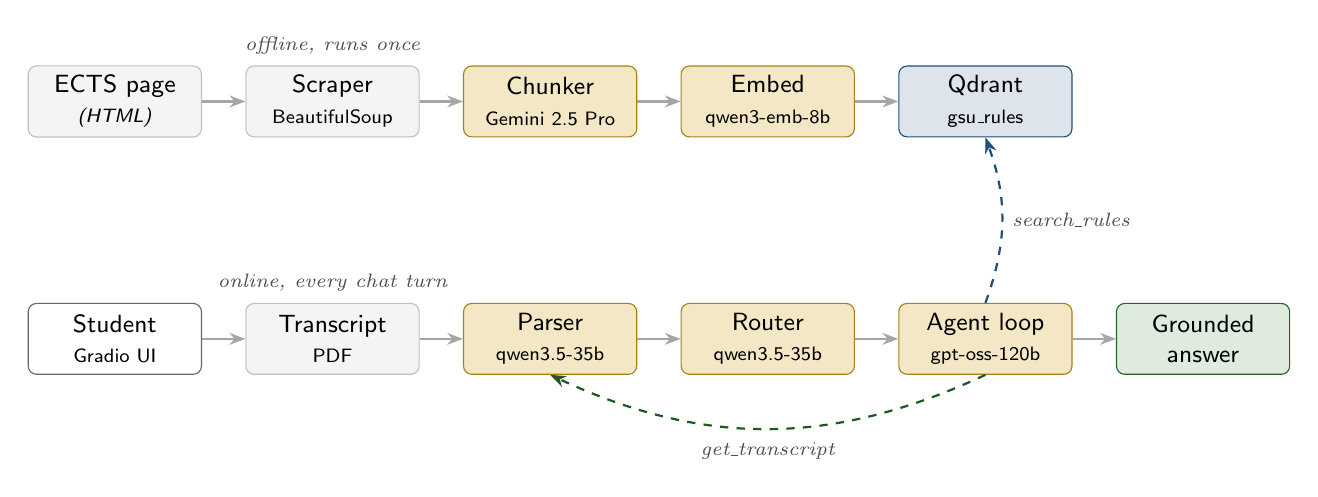
\begin{tikzpicture}[
    node distance=0.55cm and 0.55cm,
    box/.style={draw, rounded corners=3pt, minimum height=0.9cm, minimum width=2.2cm,
                align=center, font=\small\sffamily, fill=white},
    src/.style={box, fill=softgray, draw=gray!50},
    llm/.style={box, fill=gsuyellow!25, draw=gsuyellow!80!black},
    db/.style={box, fill=gsublue!15, draw=gsublue},
    outbox/.style={box, fill=accentgreen!15, draw=accentgreen!80!black},
    user/.style={box, fill=white, draw=black!60},
    arr/.style={-{Stealth[length=2mm]}, thick, gray!70},
    lbl/.style={font=\scriptsize\itshape, gray!60!black}
]

% --- Offline lane (top) ---
\node[src] (page) {ECTS page \\ \scriptsize\textit{(HTML)}};
\node[src, right=of page] (scrape) {Scraper \\ \scriptsize BeautifulSoup};
\node[llm, right=of scrape] (chunker) {Chunker \\ \scriptsize Gemini 2.5 Pro};
\node[llm, right=of chunker] (embed) {Embed \\ \scriptsize qwen3-emb-8b};
\node[db, right=of embed] (qdrant) {Qdrant \\ \scriptsize gsu\_rules};

\draw[arr] (page)    -- (scrape);
\draw[arr] (scrape)  -- (chunker);
\draw[arr] (chunker) -- (embed);
\draw[arr] (embed)   -- (qdrant);

\node[lbl, above=0.02cm of scrape] {offline, runs once};

% --- Online lane (bottom) ---
\node[user, below=2.1cm of page] (user)     {Student \\ \scriptsize Gradio UI};
\node[src,  right=of user]      (pdf)      {Transcript \\ \scriptsize PDF};
\node[llm,  right=of pdf]       (parser)   {Parser \\ \scriptsize qwen3.5-35b};
\node[llm,  right=of parser]    (router)   {Router \\ \scriptsize qwen3.5-35b};
\node[llm,  right=of router]    (agent)    {Agent loop \\ \scriptsize gpt-oss-120b};
\node[outbox, right=of agent]   (ans)      {Grounded \\ answer};

\draw[arr] (user)   -- (pdf);
\draw[arr] (pdf)    -- (parser);
\draw[arr] (parser) -- (router);
\draw[arr] (router) -- (agent);
\draw[arr] (agent)  -- (ans);

\node[lbl, above=0.02cm of pdf] {online, every chat turn};

% Agent calls tools: rules (Qdrant) + transcript (cache)
\draw[arr, dashed, gsublue] (agent.north) to[bend right=20] node[lbl, midway, right] {search\_rules} (qdrant.south);
\draw[arr, dashed, accentgreen!70!black] (agent.south) to[bend left=25] node[lbl, midway, below=0.05cm] {get\_transcript} (parser.south);

\end{tikzpicture}
\caption{Two pipelines, meeting at the agent. Solid arrows: data flow.
Dashed arrows: tool calls invoked dynamically by the agent at inference time.}
\label{fig:arch}
\end{figure}

\paragraph{Offline ingestion (runs once when rules change).} The scraper
(\texttt{src/ingestion/scraper.py}) fetches the ECTS programme page and strips
noise (scripts, navs, footers, cookie banners) using BeautifulSoup. The LLM
chunker (\texttt{src/ingestion/chunker.py}) hands the cleaned HTML to Gemini~2.5
Pro under a strict Pydantic schema (\texttt{response\_mime\_type = application/json},
\texttt{response\_schema = list[RuleChunk]}, \texttt{temperature = 0}), producing
self-contained Turkish rule sentences tagged with topic and course code. The
indexer (\texttt{src/ingestion/qdrant\_push.py}) embeds each chunk with
\texttt{qwen3-embedding-8b} (4096-d) and upserts to a Qdrant Cloud collection
with cosine distance.

\paragraph{Online serving (every chat turn).} The user lands on a Gradio UI
(\texttt{app.py}) and optionally uploads a transcript. The file is MD5-hashed
and cached in-process (capped at 50 entries to prevent leaks on the shared
HF~Space). The parser (\texttt{src/tools/transcript\_parser.py}) extracts text
with \texttt{pypdf} and asks \texttt{qwen3.5-35b} (Kloudeks) to emit a strict
JSON: GPA, total credits, failed and passed courses. A router classifies the
message as chit-chat (answered directly) or academic (delegated to the agent).
The agent loop runs \texttt{gpt-oss-120b} with two tools:
\texttt{search\_graduation\_rules} (Qdrant similarity, top-$k$=10, score
threshold 0.45) and \texttt{get\_student\_transcript} (parsed JSON). The loop is
hard-capped at 4 iterations.

\paragraph{Deployment.} Gradio and a FastMCP server are mounted into the same
FastAPI process on port 7860; the MCP endpoint is at \texttt{/mcp/sse}.
Dockerised, CI/CD'd to a Hugging Face Space. Every router call, tool execution,
and agent generation is wrapped with Langfuse's \texttt{@observe}, with
\texttt{session\_id} propagated via \texttt{propagate\_attributes} so each
browser session is one coherent trace.

\section{What is special about our design}

Five things genuinely differentiate this from the standard
``LangChain + Chroma + PDF loader'' template:

\begin{enumerate}[leftmargin=*, itemsep=0.2em]
    \item \textbf{No LangChain.} We use the native OpenAI-compatible SDK and the
          new \texttt{google-genai} SDK directly. The whole codebase fits in
          under 1k lines of Python and the agent loop is roughly 40 lines.
          Tracing and debugging are dramatically cleaner.
    \item \textbf{LLM-driven semantic chunking.} Rules in the ECTS page are
          scattered across \texttt{<td>} cells and tiny ``Not~1, Not~2''
          footnotes. Naive splitters mangle them. Letting Gemini read the entire
          HTML and emit Pydantic-validated standalone sentences was the change
          that most visibly affected retrieval quality during development:
          before the switch the retriever was returning fragments of tables;
          after the switch it returned coherent rule sentences. We do not put
          a number on the magnitude of that change for the reasons set out in
          Section~\ref{sec:bench}.
    \item \textbf{Privacy-aware model routing.} Transcript parsing goes through
          Kloudeks (Turkey-hosted); the public rule base only touches Google
          Gemini, and only during offline ingestion. Personal data never leaves
          the country.
    \item \textbf{Live MCP server, not just a chatbot.} The same tools the
          in-house agent uses are exposed via SSE at \texttt{/mcp/sse}, so any
          MCP-compatible client (Claude Desktop, Cursor, Claude Code) can query
          the GSU rule base remotely with a one-line config. This was not in the
          original spec --- once the tools existed, adding it was almost free.
    \item \textbf{Externalised prompts + hard memory ceilings.} Prompts live in
          \texttt{src/config/prompts.yaml} with Langfuse override, so we tune
          the agent without redeploying. The transcript cache is MD5-keyed and
          capped at 50 entries to keep the deployed Space stable.
\end{enumerate}

\section{Algorithms used --- and why}

\begin{table}[h!]
\centering
\small
\begin{tabular}{@{}llp{8.5cm}@{}}
\toprule
\textbf{Layer} & \textbf{Choice} & \textbf{Why this and not something else} \\
\midrule
Embedding   & \texttt{qwen3-embedding-8b} (4096-d) & The only embedding model the
              Kloudeks tenancy exposes to us. Because routing embeddings (and
              transcripts) through a Turkey-hosted provider is a hard privacy
              requirement, this was effectively a constraint, not a comparison
              \emph{won}. We did not benchmark non-Kloudeks alternatives. \\
Vector DB   & Qdrant Cloud, cosine & Managed; payload filtering by topic/rule
              type; modern \texttt{query\_points} API with native score
              thresholds. \\
Chunker     & Gemini 2.5 Pro, structured output & Long context window swallows
              the whole ECTS page; constrained decoding kills the
              ``model wrapped JSON in markdown'' bug class. \\
Parser/Router & \texttt{qwen3.5-35b} (Kloudeks) & Narrow JSON-emission tasks ---
              the 120B model would be wasteful in both cost and latency. We did
              also try a Qwen \emph{reasoning} model on this layer; see
              Section~\ref{sec:bench}. \\
Agent       & \texttt{gpt-oss-120b} (Kloudeks) & Reliable OpenAI-style tool
              calling; chains transcript $\times$ rule lookups correctly. The
              largest chat model the Kloudeks tenancy gave us. \\
\bottomrule
\end{tabular}
\caption{Per-layer model choices.}
\end{table}

\paragraph{Why an agent loop, not single-shot RAG?} Most non-trivial questions
require \emph{both} sources. ``Do I have enough technical electives?'' needs
the rule (\emph{``you need $X$ ECTS''}) and the transcript (\emph{``the student
has $Y$''}). A single-shot retrieve-then-answer pipeline cannot decide which
store to hit, let alone both. The agentic loop lets the model fetch what it
actually needs, in the order it needs it, and we can see it doing so in the
Langfuse trace.

\section{The data}

\paragraph{Source 1 --- ECTS regulations.} Scraped from
\url{https://ects.gsu.edu.tr/tr/program/programmedetails/12}. The cleaned HTML is
roughly 200~kB, which Gemini chunks into about 150 standalone Turkish rule
sentences, each 30--100 words. Topics span first-semester compulsory courses,
foreign language exemption, internship duration, technical-elective quotas, and
graduation prerequisites. Every chunk carries \texttt{topic},
\texttt{related\_course\_code} (or \texttt{GENERAL}), and \texttt{rule\_type}.

\paragraph{Source 2 --- student transcripts (PDF, runtime).} Two flavours in the
wild: the Galatasaray-issued bureaucratic PDF and the e-devlet PDF. The latter
has a known quirk --- it reports credits even for failed (F / IA / NP) courses
--- which we explicitly correct for in both the parser prompt and a
deterministic post-processing pass.

\paragraph{Schema after parsing.} The transcript collapses to a compact JSON:

\begin{lstlisting}
{
  "total_credits_completed": 192.0,
  "gpa": 3.12,
  "failed_courses":     [{"code": "INF112", "grade": "F"}],
  "all_passed_courses": [{"code": "MAT101", "credits": 6.0}, ...]
}
\end{lstlisting}

Small enough to drop verbatim into any subsequent prompt context, which matters
because the agent re-injects it when needed.

\section{Related work in the literature}

The general pattern --- retrieval grounding for an LLM --- comes from the
original RAG paper (Lewis et al., 2020). For academic advising specifically,
recent work and products group into three families:

\begin{itemize}[leftmargin=*, itemsep=0.2em]
    \item \textbf{Pure vector-DB RAG advisors} (the ``CourseGPT''/AskUni/EduBot
          family). Split FAQ documents into $\sim$500-token chunks, embed,
          retrieve top-$k$, stuff into prompt. Adequate for ``what is the
          add-drop deadline''-style questions; fails the moment the answer
          requires \emph{your} data.
    \item \textbf{Structured curriculum planners} (DegreeWorks; many in-house
          tools at US universities). Every rule hand-coded in a rule engine;
          the transcript parsed by a fixed regex pipeline. Robust, but each new
          rule means shipping code.
    \item \textbf{Agentic systems with tool calling.} ReAct-style agents
          (Yao et al., 2023) plus OpenAI's function-calling spec. The closest
          analogue to our work; public examples combine a SQL tool over a
          course catalogue with a vector tool over the policy text. Our
          contribution within this family is the combination of LLM-driven
          semantic chunking, privacy-aware model routing, and an MCP surface.
\end{itemize}

For Turkish embeddings the typical contenders are
\texttt{multilingual-e5-large}, \texttt{BGE-M3}, and the Qwen3 family. In
practice the privacy constraint forced our hand: the Kloudeks tenancy only
exposes one embedding model, so we did not compare these head-to-head ---
see Section~\ref{sec:bench}.

\section{Benchmarks and results}
\label{sec:bench}

\paragraph{We did not run a benchmark.} The Kloudeks tenancy available to us
exposes exactly one embedding model (\texttt{qwen3-embedding-8b}) and two
chat-capable models (\texttt{gpt-oss-120b} and \texttt{qwen3.5-35b}). Notably
absent: any vision-language model. Our original plan for the transcript
pipeline was to feed the rendered PDF pages directly to a VLM and skip
\texttt{pypdf} entirely --- transcript layouts are visually structured, and a
VLM would have been the cleaner tool --- but with no such model exposed on
the tenancy, we stayed with text extraction. The privacy constraint that put
us on Kloudeks in the first place rules out dropping in a non-Kloudeks
alternative just to populate a comparison row. With one realistic option per
layer, there is no like-for-like benchmark to run, so we are leaving the
section descriptive rather than tabular.

\paragraph{One thing we did try, and can speak to.} At one point we swapped the
router and parser onto a Qwen \emph{reasoning}-style model exposed via the same
Kloudeks endpoint, on the assumption that ``smarter'' parsing would help. The
opposite happened: end-to-end response time jumped by roughly \textbf{+600~s
per turn}, because the reasoning model's deliberation phase fired twice in
sequence (once in the parser, once in the router) before the agent itself even
started generating. We reverted both layers to \texttt{qwen3.5-35b}. It is a
single data point and not a controlled experiment, but it is real, and it is
the reason the architecture uses a non-reasoning model at the narrow-task
layers.

\paragraph{What we can vouch for qualitatively.} The system has been exercised
end-to-end against both an e-devlet PDF and a Galatasaray-issued transcript.
The agent reliably chains \texttt{search\_graduation\_rules} and
\texttt{get\_student\_transcript} on questions that require both sources ---
this is observable, turn by turn, in the Langfuse trace. Latency on a warm
turn sits around 4--7~s, dominated by the 120B generation step; a cold
transcript upload adds 5--8~s for parsing. The score threshold of 0.45 (vs.\
the default 0.0) was set by eye after watching low-score retrievals come back
clearly off-topic --- a hand-tuned default, not a formally-swept one.

\section{What went wrong along the way}

A non-exhaustive log, because being honest about the bumps is more useful than
pretending it worked first try:

\begin{itemize}[leftmargin=*, itemsep=0.15em]
    \item \textcolor{accentred}{\textbf{Naive chunking destroyed retrieval.}}
          The first version used a recursive character splitter on raw HTML.
          Embeddings looked plausible in isolation but the chunks were
          fragments of tables. Replaced with the Gemini chunker.
    \item \textcolor{accentred}{\textbf{Qdrant \texttt{search} deprecated mid-project.}}
          We chased a flaky warning for an evening before migrating to
          \texttt{query\_points} (commit \texttt{6818cb2}).
    \item \textcolor{accentred}{\textbf{Langfuse v3 $\rightarrow$ v4 broke tracing.}}
          \texttt{propagate\_attributes} has different semantics than the old
          \texttt{trace} helper. Rewired in \texttt{a086404}.
    \item \textcolor{accentred}{\textbf{Tool-call hallucinations.}} Early on,
          the agent would invoke \texttt{get\_student\_transcript} four times
          in a row, or call \texttt{search\_graduation\_rules} with an empty
          string. We added explicit ``red line'' prompt rules and a hard
          4-iteration cap.
    \item \textcolor{accentred}{\textbf{Markdown JSON fences.}} The parser
          occasionally wrapped its output in \texttt{```json}. A
          \texttt{re.DOTALL} extractor fishes the JSON body out as
          belt-and-braces.
    \item \textcolor{accentred}{\textbf{Memory leak on the HF Space.}} Without
          a cap, the transcript cache slowly ate Space RAM because each upload
          became a new tempdir path. MD5-keyed + 50-entry ceiling
          (\texttt{19b8bb2}) made the leak go away.
    \item \textcolor{accentred}{\textbf{e-devlet transcripts lie about credits.}}
          Failed (F / IA / NP) courses still show credits in the PDF. The
          parser used to count them; we now compensate in both the prompt and
          a deterministic post-processing step.
    \item \textcolor{accentred}{\textbf{Empty queries spinning up a full loop.}}
          Whitespace-only messages still kicked off the agent. Patched in
          \texttt{b730e62}.
    \item \textcolor{accentred}{\textbf{Live deployment blocked by an
          IP-allowlist issue (network-side).}} Locally the full pipeline works
          end-to-end without issues: parser, router, agent loop, Qdrant
          retrieval, MCP server, everything. On the Hugging Face Space,
          however, the Kloudeks endpoint consistently rejects our outbound
          requests --- our best read is that the Space's egress shows up as a
          non-allowlisted (effectively private/cloud) IP from Kloudeks'
          perspective. The code, the prompts, the tools, the traces, the MCP
          surface --- all demonstrable locally. The production endpoint is
          dark until network allowlisting is sorted on Kloudeks' side; the
          fix lives outside our codebase.
\end{itemize}

\section{What could be done next}

\begin{itemize}[leftmargin=*, itemsep=0.15em]
    \item \textbf{Full graduation checklist view.} Deterministic, template-based
          render of every requirement and its status. The data is already there;
          this is purely a UI layer on top of existing tools.
    \item \textbf{Multi-department support.} The ingestion pipeline is generic;
          adding Industrial or Electrical Engineering is mostly a scraper URL
          and a chunk-level department label.
    \item \textbf{Cross-encoder re-ranker} (e.g.\ \texttt{bge-reranker-v2-m3})
          on top-$k$ retrieval --- a standard next step for cutting the
          remaining off-topic hits we still see by eye.
    \item \textbf{An actual eval set.} A few-dozen queries reviewed with senior
          students, with ground-truth answers we can re-run on every change.
          We do not have this yet --- which is exactly why Section~\ref{sec:bench}
          is honest about not having a benchmark to report.
    \item \textbf{Token streaming.} Kills the 4--7~s silence per turn at zero
          technical cost.
    \item \textbf{User accounts.} The cache is process-global and resets on
          redeploy; a tiny user store would skip re-uploads.
    \item \textbf{Course-recommendation tool.} ``Which electives next semester
          get me to graduation fastest?'' is a constraint-satisfaction problem
          on top of the same data --- expose a planner as another agent tool.
    \item \textbf{Hardening the MCP surface.} Auth + per-client rate limits
          before any public production deploy.
\end{itemize}

\section*{Closing}

What began as ``a RAG chatbot for graduation rules'' ended up teaching us
considerably more about \emph{where} the LLM stack tends to break than about
LLMs themselves. Model choice mattered, but structural choices ---
semantic chunking, agentic tool calling instead of single-shot RAG,
externalised prompts, and hard caps on both loops and caches --- mattered more.

\vspace{0.6em}
\noindent\rule{\linewidth}{0.4pt}\\
\small Source code: \url{https://github.com/hamzayakar/gsu-advisor} \quad
Live demo: \url{https://hamzayakar-gsu-advisor.hf.space} \quad
MCP endpoint: \texttt{/mcp/sse}

\end{document}
